% Shared paragraphs between abstract and introduction

% For readibilty of latex source original pargraphs are not removed
% but moved + commented out

\newcommand{\paragi}{ This thesis describes the work that consists in
  certifying a part of a C/C++ program called \simsoc (Simulation of
  System on Chip)~\cite{helmstetter2008simsoc}, which simulates the
  behavior of embedded systems architectures based on processors such
  as ARM, PowerPC, MIPS or SH4.  }

\newcommand{\paragii}{
A system on chip simulator can be used for software development of a
specific embedded system, to shorten the development and test
phases, especially when, as is the case for \simsoc, it offers a
realistic simulation speed (about 100 Millions of instructions per
second per individual core).  Simulation makes it possible to reduce
development time and development cost, allowing for co-design
engineering, and possibility for the software engineers to run fast
iterative cycles without requiring a hardware development board.
}
\newcommand{\paragiia}{
Then a critical issue is: does the simulator actually simulate the real
hardware?  In our work, we aim at proving a significant part of
the correctness of \simsoc in order to support the claim that the
implementation of the simulator and the real system will exhibit the
same behavior.  Then a \simsoc user can trust the simulator,
especially in very critical uses.
}

\newcommand{\paragiii}{ Considering only one module in \simsoc, namely
  the ARM simulator, it somehow encodes the 1138 pages of the ARM
  reference manual in C++.  The whole simulator, which simulate ARM
  and PowerPC architecture, includes about 60,000 lines of C++ code.
  The software is very large and complicated with many complex
  features from SystemC library, and optimizations to achieve high
  simulation speed.  The first implementation of \simsoc ARM simulator
  was manually coded.  Then, mistakes in the hand written code are
  unavoidable and difficult to find due to the complexity.  Not only
  speed, but also \emph{accuracy} is highly required.  All simulated
  instructions must behave exactly like what is described in the
  specification (assuming the real hardware is conformant to the
  specification).  From the experiments performed on \simsoc, bugs
  bringing a wrong behavior were observed from time to time but it was
  hard to reveal where they were.  Using intensive tests can cover
  most of the instructions, but still left some untested rare cases of
  instructions, which lead to potential problems.  }

\newcommand{\paragiv}{
Therefore, a better approach is required to gain confidence in the
correctness of the simulator. Our proposal is to certify the simulator
\simsoc using formal methods.
}

\newcommand{\paragv}{
In this thesis, we consider one of the modules in \simsoc:
the ARM architecture simulator.
ARM architecture is one of the most popular processor design
in the embedded systems market, in particular mobile phones
and tablets.
}

\newcommand{\paragvi}{
Before taking all features of the ARM simulator into account,
we decided to focus on the basic parts,
which are the most important and sensitive:
the CPU part of the ARM architecture
(such as used by the ARM11 processor family).
}

\newcommand{\paragvii}{
In order to get the required flexibility and accuracy,
we wanted to experiment a more direct approach
based on a general proof assistant such as Coq.
Fortunately,
an operational semantics formalized in Coq of a large enough subset
of the C language happened to be available
from the \compcert project.
We then decided to base our correctness proofs on this technology.
Up to our knowledge,
this is the first development of formal correctness proofs based
on operational semantics, at least at this scale.
}

\newcommand{\paragviii}{
In this work we developed a correctness proof of a part of the hardware simulator \simsoc.
This is not only an attempt to certify a simulator, but also a new
experiment on the certification of non-trivial programs written in C.
}

\newcommand{\paragix}{
We provide a formalized representation of the ARM instruction
set and addressing modes in Coq,
using an automatic code generator
from the instruction pseudo-code in the ARM reference manual.
We also generate a Coq representation of a corresponding simulator in C,
called \simlight,
using the abstract syntax defined in \compcert.
}

\newcommand{\paragx}{
From these two Coq representations,
we can then state and
prove the correctness of \simlight,
using the operational semantics of C provided by \compcert.
}
\newcommand{\paragxi}{
Currently, proofs are available for at least one instruction
in each category of the ARM instruction set.
}

\newcommand{\paragxii}{
During this work, we improved the technology available in Coq
for performing \emph{inversions},
a kind of proof steps which heavily occurs in our setting%
}

\chapter*{Abstract\markboth{Abstract}{}}
\addcontentsline{toc}{chapter}{Abstract}

This thesis introduces the work of certifying a part of a C/C++ program
called \simsoc (Simulation of System on Chip),
which simulates the behavior of architectures based on a processor
such as ARM, PowerPC, MIPS or SH4.


\paragii

\simsoc is a complex software, including about 60,000 lines of C++ code,
many complex features from SystemC library, and optimizations
to achieve high simulation speed.
The subset of \simsoc dedicated to the ARM processor,
one of the most popular processor design,
somehow translates in C++ the contents of
the ARM reference manual, which is 1138 pages long.
Mistakes are then unavoidable for such a complex application.
Indeed, some bugs were observed even after the previous version of \simsoc,
for ARMv5, was able to boot linux.

\paragiia

We focused our efforts on a critical part of \simsoc:
the instruction set simulator of the ARMv6 architecture,
which is considered in the current version of \simsoc.


Approaches based on axiomatic semantics
(typically, Hoare logic)
are the most popular for proving the correctness of imperative programs.
However, we prefered to try a less usual but more direct approach,
based on operational semantics:
this was made possible in theory
since the development of an operational semantics for the C language
formalized in Coq in the \compcert project,
and allowed us to use the comfortable logic of Coq,
of much help for managing the complexity of the specification.
Up to our knowledge,
this is the first development of formal correctness proofs based
on operational semantics, at least at this scale.

\paragix

\paragx
\paragxi

\paragxii.

\selectlanguage{french}
\chapter*{Résumé\markboth{Résumé}{}}
\addcontentsline{toc}{chapter}{Résumé}

Cette thèse expose nos travaux de certification d'une partie d'un programme C/C++
nommé \simsoc (Simulation of System on Chip), %~\cite{helmstetter2008simsoc},
qui simule le comportement d'architectures basées sur des processeurs
tels que ARM, PowerPC, MIPS ou SH4.

Un simulateur de \emph{System on Chip} peut être utilisé pour developper
le logiciel d'un système embarqué spécifique, afin de raccourcir les phases
des développement et de test, en particulier quand la vitesse de simulation
est réaliste (environ 100 millions d'instructions par seconde par c{\oe}ur
dans le cas de \simsoc).
Les réductions de temps et de coût de développement obtenues se traduisent
par des cycles de conception interactifs et rapides,
en évitant la lourdeur d'un système de développement matériel.

%
\simsoc est un logiciel complexe,
comprenant environ 60\:000 de C++,
intégrant des parties écrites en SystemC et
des optimisations non triviales pour atteindre une grande vitesse de simulation.
%
La partie de \simsoc dédiée au processeur ARM,
l'un des plus répandus dans le domaine des SoC,
transcrit les informations contenues
dans un manuel épais de plus de 1000 pages.
Les erreurs sont inévitables à ce niveau de complexité,
et certaines sont passées au travers des tests intensifs
effectués sur la version précédente de \simsoc pour l'ARMv5,
qui réussissait tout de même à simuler l'amorçage complet de linux.

Un problème critique se pose alors : le simulateur simule-t-il effectivement
le matériel réel ?
Pour apporter des éléments de réponse positifs à cette question,
notre travail vise à prouver la correction d'une partie significative
de \simsoc, de sorte à augmenter la confiance de l'utilisateur en ce similateur
notamment pour des systèmes critiques.

% \newcommand{\paragiii}{
% Considering only one module in \simsoc, namely the ARM simulator,
% it somehow encodes the 1138 pages of the ARM reference manual in C++.
% The whole simulator, which simulate ARM and PowerPC architecture,
% includes about 60,000 lines of C++ code.
% The software is very large and complicated with
% many complex features from SystemC library, and optimizations
% to achieve high simulation speed.
% The first implementation of \simsoc ARM simulator was manually coded.
% Then, mistakes in the hand written code are unavoidable and difficult to find
% due to the complexity.
% Not only speed, but also \emph{accuracy} is highly required.
% We need all instructions to behave exactly like what is described in
% the specification.
% From the experiments performed on \simsoc, bugs bringing a wrong
% behavior were observed from time to time but it was hard to reveal where
% they were.
% Using intensive tests can cover most of the instructions,
% but still left some untested rare cases of instructions,
% which lead to potential problems.
% }

% Ce travail s'est effectué dans le cadre de
% la version suivante du logiciel, intégrant l'ARMv6.
% l'équipe \simsoc a décidé d'expérimenter l'utilisation de
% \emph{méthodes formelles} pour atteindre un meilleur degré de confiance.
% C'est précisément l'objet de notre thèse.
Nous avons concentré nos efforts sur un composant particulièrement sensible
de \simsoc:
le simulateur du jeu d'instructions de l'ARMv6,
faisant partie de la version actuelle de \simsoc.

Les approches basées sur une sémantique axiomatique
(logique de Hoare par exemple)
sont les plus répandues en preuve de programmes impératifs.
Cependant, nous avons préféré essayer une approche
moins classique mais plus directe,
basée sur la sémantique opérationnelle de C:
cela était rendu possible en théorie depuis la formalisation
en Coq d'une telle sémantique au sein du projet \compcert
et mettait à notre disposition toute la puissance de Coq pour
gérer la complexitité de la spécification.
À notre connaissance,
au delà de la certification d'un simulateur,
il s'agit de la première expérience de preuve de correction
de programmes C à cette échelle basée sur la sémantique opérationnelle.

Nous définissons une représentation du jeu d'instruction ARM
et de ses modes d'adressage formalisée en Coq,
grâce à un générateur automatique prenant en entrée
le pseudo-code des instructions issu du manuel de référence ARM.
Nous générons également l'arbre syntaxique abstrait \compcert
du code C simulant les mêmes instructions au sein de \simlight,
une version allégée de \simsoc.

À partir de ces deux représentations Coq,
nous pouvons énoncer
et démontrer la correction de \simlight,
en nous appuyant sur la sémantique opérationnelle définie dans \compcert.
Cette méthodologie a été appliquée à au moins une instruction
de chaque catégorie du jeu d'instruction de l'ARM.

Au passage, nous avons amélioré la technologie
disponible en Coq pour effectuer des \emph{inversions},
une forme de raisonnement utilisée intensivement
dans ce type de situation.

\selectlanguage{english}
\chapter{Introduction}

\section{Certification of SimSoC}
\label{sec:cersimsoc}
%\jf{What is \simsoc in less than 1/2  pg}


\paragi

% This thesis introduces the work of certifying a part of a C/C++ program
% called \simsoc (Simulation of System on Chip)~\cite{helmstetter2008simsoc},
% which simulates the behavior of architectures based on a processor
% such as ARM, PowerPC, MIPS or SH4.

\paragii

\paragiia

% Proposed by VJ
% A system on chip simulator can be used for software development of a
% specific embedded system, to shorten the developing and testing
% phases, especially when, as is the case for \simsoc, it offers a
% realistic simulation speed (about 100 Millions of instructions per
% second per individual core).  Simulation makes it possible to reduce
% development time and development cost, allowing for co-design
% engineering, and possibility for the software engineer to run fast
% iterative cycles without requiring a hardware development board.  Then
% a critical issue is: does the simulator really simulate the real
% hardware?  In our work, we aim at to proving a significant part of
% the correctness of \simsoc in order to support the claim that the
% implementation of the simulator and the real system will exhibit the
% same behavior.  Then a \simsoc user can trust the simulator,
% especially in very critical uses.

% Proposed by JF
% A system on chip simulator can be used for software development
% on a specific embedded system,
% to shorten the developing and testing phases,
% especially when, as is the case for \simsoc,
% it offers a realistic simulation speed
% (over 10 Millions of instructions per second per individual core).
% An important advantage of simulation is the reduction of developing expenses.
% Then the problem is: does the simulator really execute as the real chip.
% Here we want to proof a significant part of the correctness of \simsoc
% in order to support the claim that the implementation of the simulator
% and the real chip will have the same behavior.
% Then a \simsoc user can trust more the simulator,
% especially in very critical uses.

% % Original version by XM
% System on chip simulator is often used for software development
% on a specific embedded system,
% to shorten the developing and testing phases, thanks to
% the realistic simulation speed
% (over 10 Millions of instructions per second per individual core)
% provided by the simulator.
% And using simulator can also reduce the developing expenses.
% So it plays a very important role in the area of embedded system.
% Then the problem is if the simulator really executes as the real chip.
% Here we want to proof the correctness of such simulator in order to
% say the implementation of the simulator satisfies to the real chip.
% Then \simsoc user can trust the simulator more in very critical uses,
% if it is certain that the simulator and the hardware will behavior the
% same.

\paragiii

%VJ
% Considering only one module in \simsoc, namely the ARM simulator,
% %% original XS Just considering
% it somehow encodes the 1138 pages of the ARM reference manual in C++.
% The whole simulator, which simulate ARM and PowerPC architecture,
% includes about 60,000 lines of C++ code.
% The %
% software
% % VJ interpretation
%  is very large and complicated with
% many complex features from SystemC library, and optimizations
% to achieve high simulation speed.
% The first implementation of \simsoc ARM simulator was manually coded.
% Then, mistakes in the hand written code are unavoidable and difficult to find
% due to the complexity.
% Not only speed, but also \emph{accuracy} is highly required.
% We need all instructions to behave exactly like what is described in
% the documentation.
% From the experiments performed on \simsoc, bugs bringing a wrong
% behavior were observed from time to time but it was hard to reveal where
% they were.
% Using intensive tests can cover most of the instructions,
% but still left some untested rare cases of instructions, which lead to potential problems.

\paragiv

% Therefore, a better way is required to gain confidence in the
% correctness of the simulator. Our proposal is to certify the simulator
% \simsoc using formal methods.

%\jf{What: correctness proof of a big pgm with a big spec}

\paragv
% In this thesis, we consider one of the modules in \simsoc:
% the ARM architecture simulator.
% ARM architecture is one of the most popular processor design.
As reported by ARM Holding company, 6.1 billion ARM-based processors
have been brought to the market in year 2010 and 95\% is used
in the smart phone market.

As mentioned, the simulator is a large amount of software.
And the specification itself is rather
complex due to the rich architecture of ARM that consists of
many components (to be detailed in Chapter~\ref{cpt:formal}).
\paragvi
% Before taking all features of the ARM simulator into account,
% we decided to focus on the basic parts,
% which are the most important and sensitive:
% the CPU part of the ARM architecture
% (which is used by the ARM11 processor family).
At the time we started our work, the ARM simulator module implemented
in \simsoc was the ARM Version 5 (ARMv5) architecture.  Instead of
applying certification for this old architecture, we decided to
anticipate the evolution of \simsoc and to work on the next version:
ARM Version 6 (ARMv6).  For reasons explained below, related to the
availability of proof technologies for C (especially \compcert), it
was more convenient to have this module written in the C language
rather than in C++.  This module called \simlight \cite{rapido11} can
run standalone, or as a component integrated in \simsoc.  It is a simplified
executable version of ARMv6 simulator.

More than 60\% of the development size of \simsoc is in the CPU part,
see Figure~\ref{fig:dev}, the remaining parts consists in memory
management (virtual memory and paging) interrupt handling and
communications with peripherals. In summary, the complexity
of the target could be reduced, but it still represents more than
10,000 lines of C code to be certified.  Moreover, the complexity of
the specification is invariant, as it is given by a heavy document,
the ARM Version 6 Architecture reference manual.

\begin{figure}
\hfil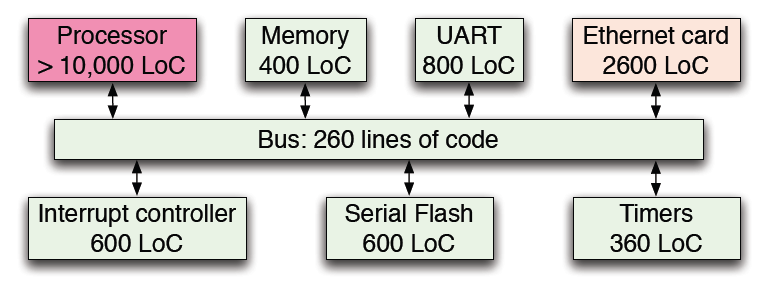
\includegraphics[width=\linewidth]{fig/develop.png}
\caption{Development size of \simsoc}
\label{fig:dev}
\end{figure}

Hence the issue at stake is how to certify a program of this size
in relation to a rather complex specification.

% This is a long term goal.
% Before going to the most intricate features of a simulator such as \simsoc,
% basic components have to be considered first.
% We then decided to focus our efforts on a sensible and important
% component of the system: the CPU part of the ARMv6 architecture
% (used by the ARM11 processor family).
% %
% This corresponds to a specific component of the \simsoc simulator,
% which was previously implementing the ARMv5 instruction set only.
% Rather than certifying this component, it seemed to us more feasible
% to design a new one directly in C, in such a way that it can be
% executed alone, or integrated in \simsoc (by including the C code in
% the existing C++ code).
% %
% We call this new component \simlight \cite{rapido11}. Combined with a small
% \texttt{main} function, \simlight can simulate ARMv6 programs as long
% as they do not access any peripherals (excepted the physical memory)
% nor coprocessors. There is no MMU (Memory Management Unit) yet. Integrating it in \simsoc just
% requires to replace the memory interface and to connect the interrupts
% (IRQ and FIQ) signals.

% \smallskip
% The present paper reports our first efforts
% towards the certification of \simlight.
% We currently have a formal description of the ARMv6 architecture,
% a running version of \simlight,
% and we are in the way of performing correctness proofs.

%% End copy

%\jf{How : not \framac, but \Compcert for 2 reasons}
%Why not \framac
%If have time, try some code from simlight with frama-c and why.
%
% Commented out by JF at the moment because it breaks the flow:
% the topic is proof, not semantics
% To provide formal semantics for a programming language, axiomatic semantics,
% operational semantics and denotational semantics are three approaches used for
% formal description.
Let us first recall that program certification is always based
on a formal model of the program under study.
Such a formal model is itself derived from a formal semantics of the
programming language.
For imperative programming languages such as C,
a popular approach is to
% Orig XM
% When talking about correctness proof of a program written in C, people will first
consider tools based on axiomatic semantics (Hoare logic),
like \framac~\cite{canet2009value}, a framework for a set of
% Orig XM
% JF -> XM: I did read anything recently on \framac,
% but what you say on "points" looks strange to me.
%
% interoperable program analyzers for C. Most of the modules integrated
% inside rely on axiomatic semantics based language ACSL (ANSI/ISO C
% Specification Language). Such specification language is powerful
% enough to express axiomatizations directly at the level of the C
% program, and define state labels that can be used to denote a program
% point in logic functions and predicates.
%
% Version by JF
interoperable program analyzers for C. Most of the modules integrated
inside rely on ACSL (ANSI/ISO C Specification Language),
a specification language based on an axiomatic semantics for C.
ACSL is powerful enough to express axiomatizations directly
at the level of the C program.
State labels can be defined to denote a program control point,
and can then be used in logic functions and predicates.
\framac is already quite a mature platform for C
program static analysis and automatic deductive verification.
% Advantage of \framac
% Version of XM
% In advantage, \framac or this kind of automatic prover is easy to use
% and requires less manpower on correctness proving of programs.  Then
% it becomes a very popular tool in this area. The axiomatic semantics
% is based on mathematical logic to prove the correctness of programs,
% which is very close related to Hoare logic.  It fits for problem
% dealing with program defined in high complexity but low complexity
% in type specification.
%
% Version of JF
An advantage of \framac or similar tools is that
it is supported by automatic proof technologies,
which save manpower consumption and
make this approach quite convenient for the user.
% %JF: said above
% Then it becomes a very popular tool in this area.
%
% %JF: other semantics too  -->  no added value here
% The axiomatic semantics is based on mathematical logic
% to prove the correctness of programs,
%
% %JF: said above
% which is very close related to Hoare logic.
%
It was successfully applied to complex and tricky programs,
e.g., Schorr-Waite algorithm, which deals with linked data structures.

% %JF: It is better to say it ij a positive way,below
% dealing with program defined in high complexity but low complexity
% in type specification.

\framac is able to perform:
\begin{itemize}
\item
  Analyzing the value of variables:
  \framac is able to compute and
  predict the range of numerical variables.
\item
  Passing the proof obligations,
  (called \emph{Verification Conditions}, VC for short)
  generated by \why~\cite{bobot2011why3}
  to automatic or interactive theorem provers.
\item
  Slicing C program into shorter ones which preserve some properties.
\item
  Navigating in C program.
\end{itemize}
%disadvantage of Frama-c
% % JF: not correct: high automation does not imply less trust per se,
% % but because the tools are far from certifiable, in contrast
% % with LCF-based provers
% % Power of the logic has nothing to do with this issue.
% % However, there is someting to say here, see below.
% However, like in general case, high automation will bring less trust.
% Because the more automatic the prover is, less powerful the logic can
% be integrated.
\label{sec:vcg}
However, in general, high automation tends to weaken the claims
for certification, as automatic provers are themselves complex,
then error-prone programs.
In theory, such programs could produce certificates which could
be checked by a reliable (e.g., LCF-based) proof assistant.
But currently it is still far from being the case.
An additional issue lies in the gap between
the axiomatic semantics used and the real implementation,
unless the VC generator is itself certified.
This issue was considered recently,
see below related work by Paolo Herms on \whyCert~\ref{sec:whycert} --
which was not available at the time we started to work
on the certification of \simsoc.

Another important issue is that automation is possible only
on theories or logics with limited expressive power.
It can make it difficult to express specifications and expected
properties at the right abstraction level,
especially in a framework where the specification is very complex.
% % JF: add a word on high complexity specifications
Currently, \framac implements a superset of first order logic.
An important current limitation for us is that
ACSL is not able to describe pointer casting.
On the contrary, the operational semantics defined for \compcert C
(to be introduced below) is able to deal with any type casting.

%Why and Why3
The \why software is one of the most important components of \framac
It is an implementation of Dijkstra's calculus of weakest preconditions.
% \jf{[SMTG to be rewritten by XM]}.
% % JF to XM; this was your original sentence, what do you mean?
% % Please take a sentence from Why/\jessie documentation.
% The previous version of Why plays the role as the platform for \framac
% plug-in \jessie front-end.
\why is the basis of the \jessie front-end, a plug-in of \framac
which compiles ACSL annotated C code into the \jessie intermediate language.
% % Version of XM
% Then the output of which goes to the VC generator of Why.
% % Version of JF
The result is given as input to the VC (Verification Conditions) generator of \why.
% % Version of XM
% At the end, the encoding result of Why can
% % Version of JF
\why then produces formulas to
be sent to both automatic provers or interactive provers like Coq.

%why3
\why version 3 is a new and completely redesigned version of \why.
It does not yet have its own front-end for C.
It has become a standard library of logical theories (integer and real
arithmetic, Boolean operations, sets and maps, etc.)  and basic
programming data structures (arrays, queues, hash tables, etc.).
%
% % Version of XM
% To adapt the new platform \why3, \jessie can now generate the intermediate
% code in \whyML, which is a rich language for specification and
% programming, in order to transmit the ACSL annotated C code into \why3
% VC generator.
%
% % Version of JF
In order to transmit ACSL annotated C code to the \why 3 VC generator,
\jessie generates an intermediate code in \whyML,
which is a rich language for specification and imperative programming.
%
% %JF: useless sentence now.
% \why3 can be seen as the reimplementation of \why.
%
% % Version of XM
% The new architecture allows encode to more language in order to
% support more new introduced automatic provers.
% Besides, a formal interface is provide for end user to ease the way
% adding new required external prover.
% So, if we depend on tool \why or \why3, we have to depend on the
% transformation line provided by \jessie and \why together, from ACSL
% annotated C code to verification condition for Coq.
%
% % Version of JF
% \jf{XM: again, I give up rewriting a sentence because I don't even
%   understand what you mean. What is ``more language''?
%  More constructs in the specification language? or another programming language
%  as input?}.
In the new architecture, the specification language is enriched in order to
support additional automatic provers.
%
Furthermore, a formal interface is provided to facilitate the
addition of new external provers.
Therefore, choosing \why or \why 3 in our case would make us depend
on the transformation chain provided by \jessie and \why together,
from ACSL annotated C code to verification conditions for Coq.


% % Version of XM
% As we mentioned before, axiomatic semantics is suitable for complex
% program but simple specification.  In the contrary, operation
% semantics is able to handle complex specifications.  In our project,
% the specification is quite complex, especially the major data type to
% express the processor state which is already defined in Section
% \ref{sec:slv6}.
% Such complex specification requires rather powerful logic.
% Usual VC generators are suitable for less complex specifications with
% simple logic.
% \hide{Every instruction operation we perform correctness
% proof is a piece of C code less than twenty lines of code. They can be
% seen as simple programs.}
% More than just compute the variation domain
% of program variables or calculate the weakest condition, we would like
% to verifying more specific properties refers to the formal ARMv6
% architecture.  Here we want to try something new and more flexible, a
% brand new way to prove our C program which represents the simulation
% of an embedded system processor ARMv6 by using the existing certified
% C operational semantics formalized in Coq specification by \compcert
% project.

% % Version of JF
In the case of \simsoc,
we need to deal both with a very large specification
including tricky features of the C language, such as type casting,
which are used in tough functions related to memory management.
In other words, we need a framework that is rich enough
to make the specification manageable,
using abstraction mechanisms for instance,
in which an accurate definition of enough features of C is available.
%
For the reasons explained above,
it was unclear that \framac would satisfy those requirements,
even with Coq as a back-end.
Automated computations of weakest preconditions
and range of variation are not relevant in our case.
We need to verify more specific properties referring
to a formal version of ARMv6 architecture.
This specification is quite complex, for instance regarding the major data type to
express the processor state (to be defined in Section~\ref{sec:slv6}).

\paragvii

% Therefore, in order to get the required flexibility and accuracy,
% we wanted to experiment a more direct approach
% based on a general proof assistant such as Coq.
% Fortunately,
% an operational semantics formalized in Coq of a large enough subset
% of the C language happened to be available
% from the \compcert project.
% We then decided to base our correctness proofs on this technology.
% Up to our knowledge,
% this is the first development of formal correctness proofs based
% on operational semantics, at least at this scale.

\section{SimSoC}
\label{sec:simsoc}

% \jf{Look at material  (reports, papers) from \simsoc, but see Chapt 3}

% \jf{Put material from current Ch. 3 somewhere in the intro.
% Explain the framework, and a little bit on the various optimizations
% performed by \simsoc.
% Was one of the original motivations.
% Will provide additional sections in the last chapter --
% further work: discuss what would the next issues when
% considering simlight3.}

% \jf{A little bit of history on Simsoc: ISS encoded by hand until v5,
% then reuse our automated chain.
% }

In this section, we introduce our certification target, \simsoc, a
Simulator of System-on-Chip that can simulate various processors at a
realistic speed.  As a simulator of System-on-Chip, its objects are
embedded system processors used in modern devices such as consumer
electronics or industrial systems (e.g. ARM, PowerPC, MIPS).  It is a
so called {\em full system simulator } because it can simulate the
entire hardware platform and run the embedded software ``as is'',
including the operating system.  Such kind of simulator plays an
important role in embedded systems development, because the embedded
software can be tested and developed on the simulator. In order to
have software and hardware ready for the market at the same time, the
software must by developed sometimes before the hardware is available.
Then a executable model of the SoC is required. A simulator also
provides additional advantages combining simulation with usage of
formal methods such as model checking or trace analysis to discover
hardware or software bugs.

Our simulator, \simsoc, works at the low-level of the system.
It takes real binary code as input and requires simulation models of the
complete board: processor, memory units, bus, network controller, etc.  It
can emulate the behavior of instruction executions, exceptions,
and peripheral interrupts.  Other than software development, it may
be used also for hardware design.  When there are additional components
provided by a third party, the software developers can test them
in the full simulation environment with modularity.

\simsoc is developed in SystemC, which is itself a C++ library, and
uses transaction level modeling (TLM) to model communications between
the simulation modules. In order to simulate processors with a
reasonably high speed, the instruction set simulation uses a technique
named {\em dynamic translation}, which translates the binary input
into an intermediate representation that is itself compiled into host
code.  Since \simsoc is a rather large and complex framework that
influences the development of both hardware and software, we have to
understand the most significant parts in order to be able to decide the
certification object.

% Systems-on-Chip (SoC), used in devices such as smart-phones, contain both
% hardware and software. A part of the software is generic and can be used with
% any hardware systems, and thus can be developed on any computer. In contrast,
% developing and testing the SoC-specific code can be done only with this SoC, or
% with a software executable model of the SoC. To reduce the time-to-market, the
% software development must start before the hardware is ready. Even if the hard-
% ware is available, simulating the software on a model provides more debugging
% capabilities. The fastest simulators use native simulation. The software of the
% target system (i.e., the SoC) is compiled with the normal compiler of the com-
% puter running the simulator, but linked with special system libraries. Examples
% of such simulators are the Android and iOS SDKs.
% In order to develop low-level system code, one needs a simulator that can
% take the real binary code as input. Such a simulator requires a model of the
% processor and of its peripherals (such as UART, DMA, Ethernet card, etc).
% When simulating a smart-phone SoC, this kind of functional simulator can be
% from 1 to 100 times slower than the real chip. These simulators have other
% uses, for example, as reference models for the hardware verification. An error in
% the simulator can then mislead both the software and the hardware engineers.
% QEMU [2] is an open-source processor emulator coming with a set of device
% models; it can simulate several operating systems. Other open-source simula-
% tors include UNISIM [1] (accurately-timed) and \simsoc [8], developed by some
% colleagues, which is loosely-timed (thus faster). Simics [12] is a commercial alter-
% native. The usual language to develop such simulators is C++, combined with
% the SystemC and OSCI-TLM libraries.

%% Begin copy from "SimSoC: A full system simulation software for embedded systems"

\subsection{Instruction Set Simulation}
\label{ssec:iss}
A full system simulator must include the instruction set
simulator, which reads the instructions of the program and exactly
emulates the behavior of the target
processor.  In order to illustrate our certification target, we
detail here the techniques to implement an instruction set simulator.  There
are three kinds of techniques implemented for \simsoc instruction
simulation, that make trade-offs between accuracy and efficiency.
They are: \textit{interpretive simulation}, \textit{dynamic
  translation with no specialization}, and \textit{dynamic translation
  with specialization}.  The \textit{interpretive simulation} is the
classical method, it includes the three stages: fetching, decoding and
executing instructions.  Although it is slow because of multiple redundant decoding
phases, it is simple to implement and reliable. It is also used as the
reference of performance for the other two techniques.  The second and
the third methods are based on dynamic translation, which uses an
intermediate representation as the decoding result.  Such intermediate
representations of decoded instructions are stored into a cache and are
re-used when the same instructions are to be re-executed.  The last
method \textit{dynamic translation with specialization} combines
dynamic translation with \textit{partial evaluation}.
\textit{Partial evaluation} specialization is a well known technique
to optimize compilation of programs.  The idea is to translate a program \emph{P}
which applies on data \emph{d} into a faster specific program
\emph{Pd}.  One can use partial evaluation in simulation to specialize
one instruction into a simpler instruction, based on data known at
decoding time. The \simsoc decoder implements partial
evaluation. At decoding time, the dynamic translation maps the binary
instructions to their partial evaluation specializations. Although
specialization of instructions results into more memory usage, it is
reasonable small compared to the memory size available on host
machines nowadays.

The technologies used in \simsoc instruction set simulation are detailed
in~\cite{ossc09}.

\subsection{Performances}

The ARM module of \simsoc used to implement the ISS of ARMv5
architecture was manually coded. The simulator is able to simulate the
commercial System-on-Chip SPEAr Plus600 circuit from ST
Microelectronics which is a dual core system based on over forty
additional components, as well as the Texas Instruments AM1705
circuit.  The simulator is able to emulate the interrupt controller,
the memory controller, the serial memory controller, the Ethernet
controller, and all peripherals which are necessary to boot Linux.
Therefore, running the Linux kernel on the SPEAr Plus simulator module
is a way of testing and debugging the simulator.  First it reads the
compressed Linux kernel binary from serial memory, uncompresses it,
then starts Linux. The booting process takes only several seconds.
The Ethernet controller can connect several simulators of the same SoC
running on the same machine or not, through TCP/IP protocol.  In
\simsoc, a mature simulator for the ARMv5 architecture has been
completed before starting our project, and two instruction set
simulators for PowerPC and MIPS were also developed.

% JF-> Vania: new subsection (moved from Ch 4), please reread
\subsection{From ARMv5 to ARMv6}
\label{ssc:arm}

% JF: moved from framework.tex (Chap 4)
% Before this development,
% The previous ARM simulator module in \simsoc was targeting the ARMv5 model
For this thesis,
we decided to consider the next version (ARMv6) of the ARM architecture,
which represented a step up in performance from ARMv5 cores.
% JF: check "step up"
ARMv6 is essentially backward compatible with ARMv5.
% they are quite different if considering the compiled program under each system.
% JF: I  don't know what to do with the previous line.
Here are the new features of ARMv6 architecture.
\begin{itemize}
\item The instruction set has been enlarged with extra instructions in
  six areas: media instruction, multiply instruction, control and DSP
  instruction, load/store instruction, architecture undefined
  instruction, and unconditional instruction.  Fortunately, all ARMv5
  mandatory instructions are ARMv6 mandatory instructions too.  For
  simulator users, application code compiled with compilers for ARMv5
  can be run over the ARMv6 simulator. If application users want to
  benefit from the new V6 instructions, they need to re-compile the
  code in the new environment.
\item The Thumb mode has changed.
  Thumb instructions of ARMv5 are not portable to
  Thumb2 (ARMv6+), nor completely backwards compatible. %JF: backward or backwards?
\end{itemize}


% Two more ISS’es are under devel-
% opment for the PowerPC and MIPS, for which the M0 and
% M1 mode have been developed, but not yet the M2 mode.
% Actually we are investigating an M3 mode that will be much
% faster using native code compilation technique.

% \subsection{The system on chip simulation}
% As a proof of concept, we have developed a simulator to
% simulate a commercially available System-On-Chip, namely
% the SPEAr Plus600 circuit from ST Microelectronics. This
% SoC contains among other components two ARM926 sub-
% systems (dual core), together with ARM UART and interrupt
% controllers, and many additional components, there are over
% 40 components in the SoC. We have developed functionally
% accurate simulators for all components directly necessary to
% boot Linux, in particular the interrupt controller, the UART,
% the Ethernet controller, the memory controller, the NAND flash
% memory controller and the serial memory controller. For other
% components that are not directly used by the Linux operating
% system, we have built stub simulation components such that
% the Linux drivers don’t crash, although the simulation is not
% accurate.
% The Linux operating system for this SoC is available from
% ST Microelectronics. Therefore it is possible to test the sim-
% ulator by running this Linux kernel binary software on the
% simulator.
% The SPEAr Plus simulator based on \simsoc simulates the
% serial memory that contains the compressed Linux boot, as the
% real device. The bootloader reads the Linux kernel from serial
% memory, uncompresses it and finally starts Linux.
% The Linux operating system then boots in a few seconds and
% networking commands such as ping can be used effectively.
% A simulated SoC can be connected to another simulator
% using TCP/IP protocol, this simulator running on the same
% machine or on a remote machine, thanks to tunneling Ethernet
% packets to the remote simulator.
% We have presented in this paper the \simsoc simulation
% framework in order to run full system simulation, with a focus
% on the ISS technology. The \simsoc framework integrates into
% a single simulation engine SystemC/TLM hardware models
% with a dynamic translation ISS designed as a TLM model,
% remaining fully SystemC compliant, requiring no further syn-
% chronization with additional outside components.
% A \simsoc ISS performs dynamic translation of the target
% code into an internal representation, using specialized func-
% tions to optimize performance. Our current developments of
% the technology are experimenting with further improvements
% of the simulation speed, in particular the idea of generating
% host machine code from the intermediate representation in a
% parallell thread. \simsoc is planned to be distributed as open
% source software.
% A complete simulator has been developed and tested for
% the ARMv5 instruction set. Two more ISS’es are under devel-
% opment for the PowerPC and MIPS, for which the M0 and
% M1 mode have been developed, but not yet the M2 mode.
% Actually we are investigating an M3 mode that will be much
% faster using native code compilation technique.

%% End copy

\section{Outline}

%\jf{Give a quick description of your work}
%Outline of the thesis
%
% % Version of XM
% At this point of the introduction, we have a summary
% of our purposes -- to certify a system on chip simulator --
% and of our framework -- how the simulator \simsoc is structured.
%
% % Version of JF
In summary, our goal is to certify (a part of) \simsoc, a system on chip simulator,
using a framework based on the operational semantics of C formalized in Coq,
and Coq itself.
%
This thesis explains our achievements in this respect.
%
Subsection~\ref{ssec:rel} discusses relevant projects which
use formal methods in the area of hardware processors,
and why we need a new approach in our experiment.
The contributions of our work are outlined in Subsection \ref{ssec:contri}.
% In order to make the thesis easier to read,
Next, Chapter \ref{cpt:bg}
provides the background on the main technologies used in our project, including a
brief introduction to operational semantics, to Coq, and to the \compcert project.
Our certification basis is the formal model of the ARMv6 instruction set simulator,
which is described in Chapter \ref{cpt:formal}.
Then the certification target, a C program for simulating the ARMv6,
is introduced in Chapter \ref{cpt:carm}.
The next chapter explains how repetitive and potentially error-prone
tasks in the production of the two previous models are automated (Chapter \ref{cpt:frame}).
Chapter \ref{cpt:correct} describes how correctness proofs are carried out.
In order to improve the performance and the management of the proofs,
we had to develop a key proof technique
for the ``inversion'' of assumptions related to
the operational semantics of C expressions,
which is described in Chapter \ref{cpt:inv}.
Chapter \ref{cpt:other} is dedicated to an additional work
using exhaustive testing for checking the coverage and correctness of
the simulator decoder.
Then we conclude in Chapter \ref{cpt:concl} and outline
future research prospects.

\section{Related work}
\label{ssec:rel}

The main difference between \simsoccert (the certification of \simsoc)
and the following projects is that we aim
at proving the correctness of a hardware simulation
whereas the target of the others is a certified hardware.
The common point is that we need a formal specification
of the instruction set of a specific processor architecture.
Different proof assistants have been used to perform the certification on the
formal model itself:
Coq in our case; ACL2, HOL, etc. in other experiments.
In our project, the formalization of the real chip ARMv6 is used
as a reference for the behavior of an ARMv6 simulator written in~C.

%\subsection*{Using ACL2 for Motorola's MC68020 and CAP}
\subsection*{Using ACL2 for embedded systems}
Researchers from Computational Logic, Inc., used ACL2
(A Computational Logic for Applicative Common Lisp)
or Nqthm (Boyer-Moore Theorem Prover)~\cite{boyer1979computational}
to specify and prove
properties of several commercial processors
as summarized in~\cite{brock1996acl2}.
ACL2 is a software system consisting of a programming language,
an extensible theory in a first-order logic,
and a mechanical theorem prover.
It can act as both an automatic theorem prover and an interactive proof assistant.
It supports automated reasoning in inductive logical theories,
which is convenient for both software and hardware verification.
Its programming language is a side-effect free extension of
Common Lisp. And it is untyped.
%
% % Commented out by JF: I don't understand and anyway, seems useless
% The functions in ACL2 is a mapping which maps each object in the
% ACL2 universe to another object in its universe.
%
The base theory of ACL2
axiomatizes its programming language semantics and its
built-in functions.
User definitions in ACL2 programming language that satisfy a definitional
principle extend the theory in a way that maintains the theory's logical
consistency.
The core of ACL2's theorem prover is based on term rewriting, and it is
extensible in the following way:
theorems discovered by the user can be used as ad-hoc proof
techniques for subsequent conjectures.

Nqthm is a theorem prover sometimes referred to as the Boyer–Moore theorem
prover.
ACL2 system is essentially a re-implemented extension of Nqthm.
We consider projects based on them together.

ACL2 and Nqthm are used to deal with different processor models in several projects.
Among them, the work for Motorola's MC68020 is very close to ours
\cite{boyer1996automated}.
% JF: transistor --> transition
% JF: No "they", see below.
% They formalized most of the user programming model of MC68020 microprocessor
A large part of the user programming model of the MC68020 microprocessor
is formalized as an abstract machine and its instruction operation as state
transitions according to its user's manual, % transistors !!
which is similar to what we did for ARMv6.
But the specification in Nqthm is formalized by hand;
no automatic generator is used.
The formal specification of the instruction set is defined
in a functional way, as in our case.
%
% % JF: No "they", see below.
% \jf{XM: are you sure that the next sentence makes sense?
% if not you are exposed to tough questions during the defence}
% An important difference is that
% fetching, decoding, and then executing an instruction
% is considered as a whole,
% where intermediate states cannot be observed.
% JF: the next sentence is redundant
% Then the state transition is not only execution of one instruction but a series
% of actions: {\it fetching}, {\it decode}, {\it execute}.
% \margxm{1}{We can also put a two dimensional picture of the user programming model of
%   ARMv6 to explain which parts we have it formalized like in automated proofs... in
%   the section explaining }
The target is the object code itself, % JF -> XM: unsure of proving target
considering that industrial strength compilers are not completely reliable;
indeed, a certified compiler generating a machine code which is
strictly equivalent to a high-level code
was not available at that time.
%is not yet invented at that time. % XM
To keep the formalized system deterministic, they abandoned the instructions
which may cause an {\it undefined} effect on the machine state.
Comparing to this,
we formalized our ARMv6 processor state differently in order to consider all
the ARM instructions, including those instructions which produce an {\it undefined} state
(see Section \ref{ssec:fsmoa}).
% JF: No "they", see below.
% They wrote the specification in the logic of Nqthm and proved their results % XM : "proved it"
The specification is written in the logic of Nqthm and proofs are obtained
using the Nqthm fully automatic theorem prover,
which cannot interact with the user once it is started.
This is totally different from the Coq proof assistant we used,
%which is completely directed by users. % version XM
where proofs are designed in constant interaction with the user.
The main theorems state that % XM: prove the correctness of:
the execution of object code terminates and the
returned machine state is considered normal,
that all registers are set to the right location and
that the effect of the execution is only on the relevant memory blocks.

% % XM
% To use fully automatic theorem prover like Nqthm, it requires less
% man-power on theorem proving but much work on specification.
%
% % JF
The use of fully automatic theorem provers like Nqthm requires less
man-power on theorem proving but much work on the specification.
Once the
formalization and the stated theorems are put in Nqthm logic system,
we expect the automatic prover to do the rest.
With this technique % XM: they
% JF -> XM : don't use "they"; instead, you can use the passive form for instance
% verified mechanically the object code produced by GNU C compiler for hundreds of
% lines of C.
the object code produced by GNU C compiler for hundreds lines of C
could be mechanically verified.

% But (XM)
Still, % JF
the gap between C and the GNU C produced object code is not solved,
because the GNU C compiler can not be considered fully trusted.
% %XM
% So this method does not produce a completely verified C program.
% JF
So this method cannot be used for providing results which would be
meaningful (and conveniently expressed) at the level of a C program.

Another project used ACL2 on the object processor CAP from Motorola company.
% They formalized the full ALU and I/O system of CAP in ACL2.
The full ALU and I/O system of CAP is formalized in ACL2.
%The syntax of ACL2 is a subset of that of Common Lisp.
The CAP implementation is a three-stage instruction pipeline; % they proved an
an appropriate correspondence between the CAP model with pipe-line and a simpler
pipeline-free one is proven. Also the implemented DSP algorithm FIR
(Finite Impulse Response) is proved to be equivalent to the formal specification.
% Another important performance for communications signal processing
% is proved correct, the ``5PEAK`` algorithm, for making sure that CAP ACL2 model
% executes the 5PEAK object code on an
% appropriate initial state for the appropriate machine cycles and the five
% highest peaks and their addresses are deposited into certain locations.
Moreover, % they enrich
the basic library for ACL2 on data structure was enriched,
for example with array, list, record, bit vector, etc.
New modules on modular arithmetic, integers, hardware operations, and so on were built.
These developments are reusable by other projects because
the definitions are not specific to the CAP model.
% Aside from making subsequent code proofs easier,
% this work had the important benefit of identifying an equivalence condition
% sufficient to avoid hazards yet weak enough to admit CAP application programs.

% JF : I comment out the next sentence:
%      I'm unsure that it is understandable and really useful
% It focuses on another level of representing the processor CAP
% rather than in the sense of instruction set simulator.

% 5peak program code,
% CAP execute on an appropriate initial state and for the appropriate machine cycles,
% the five highest peaks and their addresses are deposited into certain locations.

% ACL2 Theorems About Commercial Microprocessors

% ACL2 stands for "A Computational Logic for Applicative Common Lisp.
% ACL2 is both a mathematical logic and system of mechanical tools which can be used to construct proofs in the logic.

% The ACL2 logic is a first-order,
% essentially quantifier-free logic of total recursive functions providing mathematical induction and two extension principles:
% one for recursive definition and one for "encapsulation."

% The syntax of ACL2 is a subset of that of Common Lisp.

% The object microprocessor is CAP from Motorola company.
% The CAP executes a 64-bit instruction word, which in the arithmetic units is further decoded into a 317-bit,
% low-level control word.
% The instruction set includes no-overhead looping constructs and automatic data scaling.

% The CAP implementation includes a three-stage instruction pipeline with many visible pipeline hazards.
% But they proved an appropriate correspondence between the pipe-lined CAP model and a simpler pipeline-free model of the CAP.
% Aside from making subsequent code proofs easier,
% this work had the important benefit of identifying an equivalence condition sufficient to avoid hazards yet weak enough to admit CAP application programs.

% They have done:
% executable CAP specification, full ALU and I/O included;
% reusable ACL2 books about modular arithmetic, logical operations on integers,
% hardware arithmetic and bit vectors, arrays, record structures, and list processing;
% Equivalence to Non-Pipelined Model;
% proved FIR filter computes correct result;
% 5peak program code,
% CAP execute on an appropriate initial state and for the appropriate machine cycles,
% the five highest peaks and their addresses are deposited into certain locations.


% (* In simlight, 'unpredictable' is defined to print error message "simulating something unpredictable"
% In COQ specification, 'unpredictable' is a definition, it returns KO result. It is not really unpredictable. *)

A very recent work used ACL2 for developing a significant subset of 
X86 instruction set~\cite{shilpi2013}.
The formal model of the X86 processor is executable and can run some binary programs.
Some small binary programs are automatically verified 
under ACL2's interactive theorem proving environment using a
symbolic execution technique. 

\subsection*{Formalized x86 in Coq}

% JF: by -> in
In a recent work done in a cooperation between Harvard University,
Lehigh University, NSF, and Google, a model of x86 has been formalized
in Coq~\cite{morrisett2012rocksalt}.  The whole project is called
Native Client (NaCl). It is a platform allowing Google's Chrome
browser users to execute native code on the browser.  A sandbox policy
is used to ensure several properties.  The most important ones are to
ensure that read/write operation on arbitrary memory blocks are only
caused by trusted code, instructions related to system calls are
avoided, and communication can only happen within well-defined entry
points.  These properties of the sandbox policy protect the system
from bugs or concurrent access to memory.  The aim of this work is to
obtain a highly trusted assurance checker for the sandbox policy.  A
checker for a 32-bit x86 (IA32) processor without floating-point
instructions, RockSalt was built.  This new achievement is better than
the original version provided by Google in three aspects: it is
faster, lighter, and more flexible.

This project has some similarities with ours: the core of RockSalt was
automatically generated from the Coq formal specification using
extraction to OCaml code; then it was manually translated in C
language in order to have an implementation for NaCl.  A new Coq model
for x86 was defined.  In the future, it is expected to support
reasoning about the behavior of x86 machine code using a verified
compiler such as \compcert.  RockSalt relies only on a DFA
(Deterministic Finite-state Automaton) encoding table and some trusted
C code.  The checker is extremely fast: 1M instructions can be checked
within one second.  Also, it has a small run-time trusted computing
base and can be integrated into NaCl runtime easily.  The formal model
of x86 ISS (Instruction Set Simulator) has the same architecture as a
translator: a decoder from binary code to an abstract syntax, a
compiler from this abstract syntax to RTL instructions; and an
interpreter for RTL instructions.  Because no predefined formal model
could be considered as a trust-base, tests were created for this
complex model, in order to gain confidence.

For validation, an executable OCaml model is extracted from the Coq
specification, and the behavior of the OCaml model is compared with
the real x86.  More than ten million binary instructions could be
simulated in around sixty hours on Intel Xeon.  Moreover, fuzz tests
are used to cover problems that cannot be considered by the previous
tests.  Fuzz test can cover all forms of one kind of instruction, and
all of them can be exercised.  The Coq processor model in this
project % is used in a different way from ours.
is essentially an intermediate specification which is used to obtain
more secure C code.  However the manual translation from extracted
OCaml code to C is not explained in~\cite{morrisett2012rocksalt}.
Tests are only used at the level of OCaml code.  Altogether, it is
unclear that the resulting C code has the same behavior as the Coq
specification. % JF: "proved correct " would be redundant


% The logic of Nqthm is a quantifier-free first order with equality.
% The Nqthm theorem prover is a mechanization of the preceding logic.
% The theorem prover is fully automatic in the sense that once a proof attempt has
% started,
% the system accepts no advice or directives from the user.
% The only way the user can interfere with the system is to abort the proof attempt.

% They have formalized most of the programming model of MC68020 microprocessor with the help of user's manual view,
% mainly focused on user available instruction set.
% But they abandoned those instructions which introduce undefined effects on state.
% How they deal with exception is to ignore the supervisor mode,
% the machine will halt when exception occurs.
% They formalizing the microprocessor as a state transition too.
% They also defined the semantics for their microprocessor model,
% and built a library of lemmas for proof.
% Their lemmas include those for arithmetic,
% alternative interpretations, machine state management.
% Their main theorem for a piece of object code program is the next state of executing such program is exactly the state they expect.
% What we have stated is the next state of a C instruction is related to the formal representation of such state.



% Ref. 1
% ACL2 Theorems About Commercial Microprocessors

% ACL2 stands for "A Computational Logic for Applicative Common Lisp.
% ACL2 is both a mathematical logic and system of mechanical tools which can be used to construct proofs in the logic.

% The ACL2 logic is a first-order,
% essentially quantifier-free logic of total recursive functions providing mathematical induction and two extension principles:
% one for recursive definition and one for "encapsulation."

% The syntax of ACL2 is a subset of that of Common Lisp.

% The object microprocessor is CAP from Motorola company.
% The CAP executes a 64-bit instruction word, which in the arithmetic units is further decoded into a 317-bit,
% low-level control word.
% The instruction set includes no-overhead looping constructs and automatic data scaling.

% The CAP implementation includes a three-stage instruction pipeline with many visible pipeline hazards.
% But they proved an appropriate correspondence between the pipe-lined CAP model and a simpler pipeline-free model of the CAP.
% Aside from making subsequent code proofs easier,
% this work had the important benefit of identifying an equivalence condition sufficient to avoid hazards yet weak enough to admit CAP application programs.

% They have done:
% executable CAP specification, full ALU and I/O included;
% reusable ACL2 books about modular arithmetic, logical operations on integers,
% hardware arithmetic and bit vectors, arrays, record structures, and list processing;
% Equivalence to Non-Pipelined Model;
% proved FIR filter computes correct result;
% 5peak program code,
% CAP execute on an appropriate initial state and for the appropriate machine cycles,
% the five highest peaks and their addresses are deposited into certain locations.


% (* In simlight, 'unpredictable' is defined to print error message "simulating something unpredictable"
% In COQ specification, 'unpredictable' is a definition, it returns KO result. It is not really unpredictable. *)

% Ref. 2
% Automated Proofs of Object Code for a Widely Used Microprocessor

% They formalized the MC68020 microprocessor with the mathematical logic of automated reasoning system Nqthm (Boyer-Moore Theorem Prover).
% And they checked the correctness of MC68020 object code programs for binary search,
% Hoare's Quick Sort,
% twenty-one functions from the Berkeley Unix C string library, and other well-know algorithms.

% Their proving is at the object code level.
% It is because the semantics of machine code must be considered if we use a particular processor;
% some parts of high-level programming languages can not be formalized and some industrial strength compilers produce erroneous code;
% higher-level languages don't take real-time analysis into account.


% The logic of Nqthm is a quantifier-free first order with equality. The Nqthm theorem prover is a mechanization of the preceding logic.
% The theorem prover is fully automatic in the sense that once a proof attempt has started,
% the system accepts no advice or directives from the user.
% The only way the user can interfere with the system is to abort the proof attempt.

% They have formalized most of the programming model of MC68020 microprocessor with the help of user's manual view,
% mainly focused on user available instruction set.
% But they abandoned those instructions which introduce undefined effects on state.
% How they deal with exception is to ignore the supervisor mode,
% the machine will halt when exception occurs.
% They formalizing the microprocessor as a state transition too.
% They also defined the semantics for their microprocessor model,
% and built a library of lemmas for proof.
% Their lemmas include those for arithmetic,
% alternative interpretations, machine state management.
% Their main theorem for a piece of object code program is the next state of executing such program is exactly the state they expect.
% What we have stated is the next state of a C instruction is related to the formal representation of such state.

\subsection*{An instruction set generator for an ideal processor}

A German project describes in ~\cite{kuhne2009generating}
an Instruction Set Simulator generation technique
which aims at generating an efficient ISS from the RTL
(Register Transfer Level) description.
The ITL (Iterative Temporal Logic) language is used to design the ISS at the
RTL level, then C++ code is generated from it.
The interval temporal logic is a combination of temporal logic and first-order logic
able to deal with sequential and parallel composition.
It includes a notion of finite sequences.
First order interval logic was first designed for formalizing and verifying hardware
protocols. It is sufficient for specifying computer-based systems, both
hardware and software.
%JF: I remove the following, because if you can deal with HO logics, you can do everything.
% but impossible for theorem proving with higher-order logics.
Some of the standard operations of VHDL or Verilog language can be expressed as
temporal logic expressions to describe the behavior of a synchronous sequential
system.

The verification of safety properties is performed using a technique
called IPC (Interval Property Checking) which is designed to check if
a model satisfies a set of properties written in a dedicated
verification language, ITL in this case.  The main idea followed here
is to use an arbitrary initial state instead
% JF: starting state may work but I'm unsure. Initial state is OK.
of the initial state of BMC (Bounded Model Checking).  Any property
that holds from an arbitrary initial state also holds from any
reachable state. Conversely, false negatives can occur in IPC. These
false negatives need to be removed by adding invariants in order to
restrict the set of initial states.  In order to gain speed for
simulation, optimizations are performed on the C++ code generation
like in any other state-of-the-art simulators by the following two
methods: first, arithmetic and simple logic operation are mapped to
corresponding native C++ operations; second, additional variables are
used to store temporary results and to cache intermediate results of
computations.  The formal verification aims at proving the equivalence
between RTL and ISA models.
% JF: better explained in your sentences below
% which needs a mapping function
% from the implementation state of the CPU to the state in ISA.
The main idea of the equivalence proof is very similar to ours
(see Chapter~\ref{cpt:correct}):
it is based on
a mapping from the RTL state representing CPU to the corresponding ISA state in C,
and on next-state transitions for both the RTL model and the ISA model of the C program.
Proving that the interface signals of the design is correctly implemented
is also performed in the same way.
For code generation, the input source is specified in VHDL.
The first experiment was achieved on an invented ideal simplified CPU model.
It contains eight 16-bit registers and a special register
used as interrupt return vector.
There are only seven instructions for logic, arithmetic, memory accessing, and jump.
For the second experiment, an industrial processor design was chosen.
It contains 64 32-bits registers and 88 instructions based on the DLX instruction
set architecture and a memory model with simple interface.
This corresponds to 10,000 lines of VHDL code,
reformulated into a 2000 lines ITL specification
to be used as the source of the C++ code generator.
Compared to \simsoc, the size of the formal specification is smaller
and with ITL specifications, less properties can be expressed and proved than with Coq.

\subsection*{A trustworthy monadic formalization of ARMv7 instruction set architecture}

The computer laboratory in Cambridge University
used HOL4 to formalize the instruction set architecture of ARMv7~\cite{FoxM10}.
The target here was to verify an implementation of this architecture
with \emph{logical gates}, whereas for \simsoc,
we consider a simulation written in C.
Reusing the work done at Cambridge was considered for \simsoc.
However, as our approach is based on \compcert,
which is itself written in Coq instead of HOL4,
it was more convenient to write our own specification.
% With the same target, the ARM instruction set, our approaches are close to each other.
% But the difference is quite obvious.
% The formalization using HOL 4 in this approach is not
% reusable in our project. Because we require the formal model of ARM architecture in Coq in order
% to link the formalized C language in Coq provided by \compcert for the C specifications of \simsoc.
The  achievements obtained at the Cambridge projects are:
\begin{itemize}
\item
  A model of the ARM instruction set architecture in the HOL language.
  Other than ARMv7 instruction set which is backward compatible with previous versions,
  the model considered here has the full support for the Thumb-2 instruction set, too.
\item Additional software for simulation, an assembler, and a disassembler in ML.
\item Automatic extraction of single step theorems from a monadic representation
  of a single ARM instruction, for evaluation.
\item
  Besides the tools and specifications formalized or derived inside HOL logic,
  some other tools that are outside HOL logic: the assembly code parser,
  the disassembler, and the encoder.
  They are considered not completely reliable.
\item The formalized model can operate on machine code level.
\item The execution results are used for comparison with the real hardware
  in order to validate the model.
\end{itemize}

The instructions have been grouped together with related ones.  This
reduces greatly the specification size. But the HOL 4 model is a little too
precise. For example, it specifies the resource accessing order when
updating the PC.
But this order is not specified in the reference manual.
% It means they have to invented it by themselves.
During validation,
three boards are used to assess the execution results.
And the tests are generated randomly by a test generator.
Additional confidence in this development was achieved
by observing the behavior of verified code,
and running the model on ARM code that calculates a non-trivial known function.
% Finally, bugs are found by validation steps. JF: removed because it is trivial
Some weaknesses are:
storing instructions are not completed;
problems happen when updating on registers PC or SP occur;
exceptions are not well handled;
tests do not cover unpredictable and undefined instruction,
which have been filtered in test generation;
the model does not include the privileged mode,
nor the instruction changing the current processor mode;
implementation dependence or system features cannot be fully tested.

\subsection*{WhyCert: A certified implementation of VC generator}
\label{sec:whycert}

Paolo Herms's Ph.D thesis \cite{herms13phd}~\cite{herms2012certified}
provides a certified
verification condition generator for several provers,
called \whyCert.
The work is also based on \compcert C operational semantics.
Using a VC generator is another way of ensuring the safety requirements of programs
written in high-level programming languages,
as mentioned in Section~\ref{sec:vcg},
as well as the importance of certifying a VC generator.
In \whyCert, the VC generator was implemented and proved sound in Coq,
then extracted to an executable OCaml program.
As suggested by the name \whyCert, this work is inspired by
\why\cite{filliatre07cav}, a platform for deductive program
verification.  To make it usable with arbitrary theorem provers as
back-ends, it is generic with respect to a logical context, containing
arbitrary abstract data types and axiomatisations.
% % JF The style needs improvement but I'm tired
This is suitable to formalized memory models needed to design
front-ends for mainstream programming language,
as it is done for C by VCC above Boogie or by \framac/\jessie above \why.
The inputs are imperative programs written in a core language
which operates on mutable variables which are typed in the logical context.
The output is made of logic formulas which are built upon the same logical context.

% % JF Ideas moved to \label{sec:vcg}
% we consider the result of Hoare
% logic approach is weak because VC generators are not certified yet
% until Paolo Herms's work came out. This work has filled the gap
% between the proof obligations free automatic provers and the certified
% program verifier.


% This thesis belongs to the domain of software verification. The goal
% of verifying software is to ensure that an implementation, a program,
% satisfies the requirements, the specification. This is especially
% important for critical computer programs, such as control systems for
% air planes, trains and power plants. Here a malfunctioning occurring
% during operation would have catastrophic consequences. There are
% numerous examples of software failures in the past. The interested
% reader may refer to a very comprehensive list composed by Nachum
% Dershowitz.1 Software requirements can concern safety or
% functioning. Safety requirements, such as not accessing memory
% locations outside valid bounds, are often implicit, in the sense that
% any imple- mentation is expected to be safe. Many high-level
% programming languages ensure the main safety requirements by providing
% to the programmer an abstraction of the machine that disallows unsafe
% operations. On the other hand low-level languages, like the C
% programming language, grant the programmer the full access to the
% machine exposing him also to the full risk. Unfortunately the use of
% low-level languages can often not be avoided – especially in the
% implementations of afore- mentioned control systems. Indeed the C
% language remains nowadays the language of choice for developing
% critical embedded software.

\subsection*{The seL4 project}

The NICTA company provides a secured microkernel seL4~\cite{klein2009sel4}, 
a member of L4 microkernel family.
The formal verification is based on the interactive theorem prover Isabelle/HOL.
The correctness proofs are established according to a 
correspondence between 
an abstract and a concrete representations of the seL4 system.
The concrete model is the C implementation,
which is translated to Isabelle using a intermediate language 
called \texttt{com},
which has an operational semantics like \compcert C.
However this language handles a smaller subset of C than \compcert C.
Unsupported features of \texttt{com} that are supported in \compcert C include:
\begin{itemize}
\item
  pointers to automatic storage
\item
  float, function pointer, union
\item
  switch, goto, break, continue
\end{itemize}
Note that for SimSoC, we need function pointer, switch, break.

\section{Contributions}
\label{ssec:contri}

\paragviii
% In this work we develop a correctness proof for the hardware simulator \simsoc.
% This is not only an attempt to certify a simulator, but also a new
% experiment on the certification of non-trivial programs written in C.
In our approach, we do not use the popular axiomatic semantics,
but the C operational semantics defined by the \compcert project.

% Our first contribution is a formalized representation of the ARM instruction
% set and addressing modes in Coq,
% %by building the first version of the automatic code generator
% using an automatic code generator
% from the instruction pseudo-code in the ARM reference manual.

% Our second contribution is the generation of the corresponding ARM instruction set
% into \compcert syntax in Coq representation.

% Having the two representations in Coq, it is ready to process the main contribution,
% proving the correctness of the C representation of ARM instruction set based
% on the operational semantics of C provided by \compcert.

% Fourth contribution is the generator of ARM instruction decoder, based also on
% the ARM instruction part of the reference manual.

% Next contribution is building a tests generator for the instruction decoder.
% It can generate massive tests to test the coverage of the ARM instruction decoder.

\paragix
% We provide a formalized representation of the ARM instruction
% set and addressing modes in Coq,
% %by building the first version of the automatic code generator
% using an automatic code generator
% from the instruction pseudo-code in the ARM reference manual.
% %
% We also generate a Coq representation of a corresponding simulator in C,
% called \simlight,
% using the abstract syntax defined in \compcert.
The text version of \simlight was previously developed
as a component of \simsoc by C. Helmstetter~\cite{rapido11}.

\paragx
Our first achievement in this direction was described in~\cite{2011first}.
\paragxi

\paragxii~\cite{2013itp}.
% From these two Coq representations,
% we can then state and
% prove the correctness of \simlight,
% using the operational semantics of C provided by \compcert.
% Our first achievement in this direction was described in~\cite{2011first}.
% Currently, proofs are available for at least one instruction
% in each category of the ARM instruction set.
% In passing, we improved the technology available in Coq for
% performing \emph{inversions},
% a kind of proof steps which heavily occur in our setting~\cite{2013itp}.

Additional contributions include
a generator of a decoder for ARM instructions,
also based on the analysis of the ARM reference manual,
and a test generator for the instruction decoder,
which can generate massive tests covering all ARM instructions.



%%% Local Variables:
%%% mode: latex
%%% TeX-master: "thesis"
%%% End:
